\subsection{Result Research}

Correlation coefficients are used in statistics to measure how strong a relationship is between two variable space. Concretely, in this case those variable space are Semantic score and RUBY. 


We aim to figure out specifics of a dataset in which RUBY can work well. Because RUBY was created to estimate the semantic of code translation, the dataset in which RUBY works well also is the dataset containing the high correlation between Semantic score and RUBY. 

\subsubsection{The Use of RANSAC}
The RANSAC (Random Sample Consensus) algorithm~\cite{ Fischler:1981:RSC:358669.358692} is a simple, yet powerful, technique that is commonly applied to the task of estimating the parameters of a model, using data that may be contaminated by outliers. RANSAC estimates a global relation that fits the data, while simultaneously classifying the data into inliers (points consistent with the relation) and outliers (points not consistent with the relation). Due to its ability to tolerate a large fraction of outliers, the algorithm is a popular choice for a variety of robust estimation problems.


RANSAC assumes that the training data consists of inliers that can be explained with the model and outliers that are gross-erroneous samples which do not fit the model at all. So using outliers when training the model would increase our final prediction error, as they contain almost no information about the model. Therefore, in our research scope, we use RANSAC as a mean of data classifier which returns a set of points contributing to the correlation of the method (inliers) and another set of points decreasing the correlation of the method (outliers).

\subsubsection{Experiments}
We conducted independtly 10 experiments with RANCSAC running on the same dataset derived from our result tested on model \textbf{XXX}. The data set contains 375 pairs representing RUBY and Semantic score caculated for the set of traslated methods of \textbf{XXX}. (Table~\ref{table:RANSAC_experiments}) shows results of our 10 experiments which contains the number of inlier points and the correlations of those inliers. The number of inliers is almost around 300 out of 375, while the figure for their correlation is at high rate between 0.93 and 0.95. 
According to the outcome, we chose the dataset result with the \textbf{median} of correlation that is the experiment No5 (correlation = 0.954874293) in the table for analyzing and finding out the specifics of that dataset. Figure~\ref{fig:inliers_outliers} shows the result of experiment No5 gained from RANCSAC.
\begin{table}
	\caption{RANSAC experiments}
	\begin{tabular}{|c|c|c|c|c|}
		\hline
		Experiment Number & Number of inliers & Correlations of inliers \\
		\hline
		10	& 315	& 0.934700727 \\		
		8	& 312	& 0.945424846 \\	
		9	& 312	& 0.947983773 \\
		4	& 310	& 0.948196013 \\
		{\cellcolor[gray]{.8}}5	& {\cellcolor[gray]{.8}}308	& {\cellcolor[gray]{.8}}0.954874293 \\
		7	& 244	& 0.955112418 \\	
		1	& 283	& 0.957661146 \\
		3	& 303	& 0.958122675 \\
		2	& 298	& 0.958659967 \\
		6	& 277	& 0.959811603 \\		
		\hline
	\end{tabular}
	\label{table:RANSAC_experiments}
\end{table}

\begin{figure}[t]
	\caption{An example: Dataset in experiment No5 classified into inlier points(green) and outlier point(yellow)}
	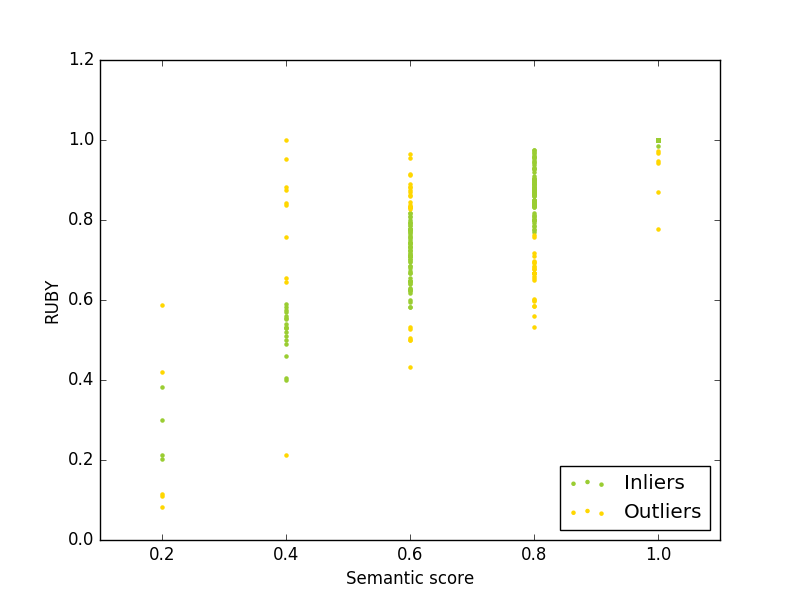
\includegraphics[scale=0.4]{img/inliers_outliers.png}
	\centering
	\label{fig:inliers_outliers}
\end{figure}

\subsubsection{Specification category}
\textbf{Inliers.} We manually classify the method set of the inlier points into serveral categories based on the relation between the method and its reference. Table~\ref{table:inliers_result} shows the result of classification for our set of data.
\textbf{TODO: Explain table}


\textbf{Outliers.} The past Stephen Hawking said: "One of the basic rules of the universe is that nothing is perfect. Perfection simply does not exist". Although RUBY metric performces the high correlation in representation semantic score, there exists cases in which RUBY does not work well. With the same manually checking method as done with inliers, the table~\ref{table:outliers_result} shows RUBY's failure in measuring semantic for those phenomenon.
\textbf{TODO: Explain table}
\begin{table}[]
	\centering
	\caption{Inlier classification}
	\label{table:inliers_result}
	\begin{tabular}{|m{1cm}|m{3cm}|m{4cm}}
		\hline
		Type      & Category         & Description                                                                                                                    
		\\
		\hline
		High RUBY & IDENTIDFIED           & Code is the same with the reference                                                                                             \\
		& SAME\_FUNC\_DIFF\_LEX & Code uses a variety expression for the same functionarity with the reference, e.g for vs foreach, array[i] vs array.get(i)\\
		& SAME\_DATA\_FLOW      & Code has the same data flow with the reference but there are still incorrect pieces of code                                     \\
		\hline
		Low RUBY  & SAME\_KEYWORDS        & Code has the same keywords with the reference, i.e API names, method calls, variables. However, their usage is incorrect           \\
		& DISORDERED            & Code has some same pieces of code with the reference. However they are disordered                                               \\
		& DIFFERENT             & Code is totally different from the reference \\
		\hline                                                                                   
	\end{tabular}
\end{table}


\begin{table}[]
	\centering
	\caption{Outlier classification}
	\label{table:outliers_result}
	\begin{tabular}{|m{1cm}|m{3cm}|m{4cm}}
		\hline
		Type      & Category         & Description                                                                                                                    
		\\
		\hline
		High RUBY &     INCOMPLETED       &  Code has a lot of syntax errors and it is not completed however it still has a majority of same piece with the reference which include unimportant information \\                                   
		\hline
		Low RUBY  & ALGORITHM\_VARIETY        & Code has the same functionarity with the reference, however it has been implemented by other algorithm, the lexical and data flow is almost different           \\
		\hline                                                                                   
	\end{tabular}
\end{table}